% Tento soubor nahraďte vlastním souborem s obsahem práce.
%=========================================================================
% Autoři: Michal Bidlo, Bohuslav Křena, Jaroslav Dytrych, Petr Veigend a Adam Herout 2019
\chapter{Úvod}

Aktuálna doba či už v závislosti od Pandémie alebo digitalizácie naučila občanov ostávať vo svojich obydliach, zatiaľ čo úradné oznamy sú buď zobrazené v neprehľadných formách na internetových stránkach alebo fyzicky na úradoch mesta.

Ich centralizácia a digitálne sprehľadnenie je nevyhnutné pre jednoduchú komunikáciu úradu a obyvateľa mestskej časti. Úlohami práce je preto integrácia dátových sád 29 častí mesta Brna, využitie geografickej polohy jednotlivých úradných dosiek a ich prepojení s obyvateľstvom.

V Teórii \ref{theory} sa práca zameriava na existujúce riešenia a stav aktuálnych poskytnutých dát.

\chapter{Teória}
\label{theory}
Táto kapitola opisuje, aké boli aktuálne riešenia ustanovenie pevnej formy dát, ich zjednotenie a následné informovanie užívateľov pomocou mobilných aplikácii.


\section{Riešenie digitalizácie úradných dosiek}

Digitálne dosky od sprostredkovateľa obec24, GROUP24 INNOVATIONS s.r.o., ktorá ponúka digitalizáciu úradných dosiek pomocou veľkoplošných obrazoviek s dotykovým displejom, pre jednoduchú navigáciu a interakciu. Takáto digitalizácia urýchľuje vystavovanie, dovoľuje rýchlym úpravám, škálovateľnosti atď. Avšak riešenia sú ponúkané a lokalizované na mestských úradom čím sa otázka dostupnosti bohužiaľ nevyriešila. Jedno z riešení Obce24 je na obrázku \ref{urednideskaobec24}.


\begin{figure}[H]
	\centering
	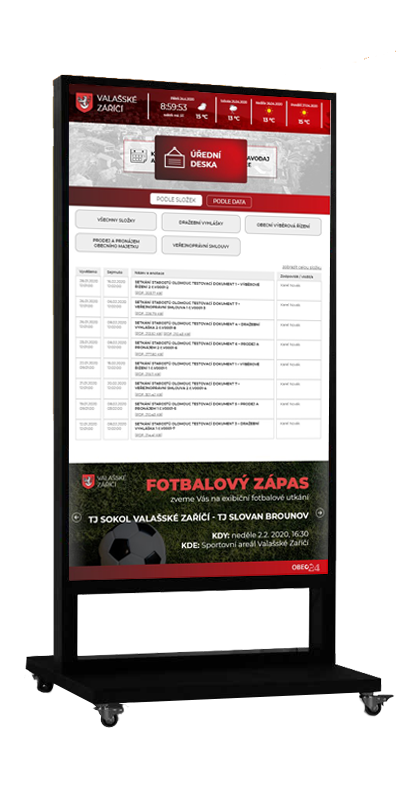
\includegraphics[width=0.25 \linewidth]{img/urednideskaobec24.png}
	\caption{MODEL i01 INDOOR
SAMOSTATNĚ STOJÍCÍ poskytujúci dotykovú obrazovku pre navigúciu v úradných doskách}
	\label{urednideskaobec24}
\end{figure}

\subsection{Notifikačná aplikácia}
Notifikácie sú prevedené pomocou aplikácie Telegram spojené s GitHub. Telegram je chatovacia služba. Je využitá z toho dôvodu, že dovoľuje jednoducho naprogramovať automatických botov, jeden už z existujúcich, ktorý umožňuje upozorniť na novo vykonanú zmenu v github projekte  \cite{notifikacniAplikace}. Notifikácia je zobrazená na obrázku 

\begin{figure}[H]
	\centering
	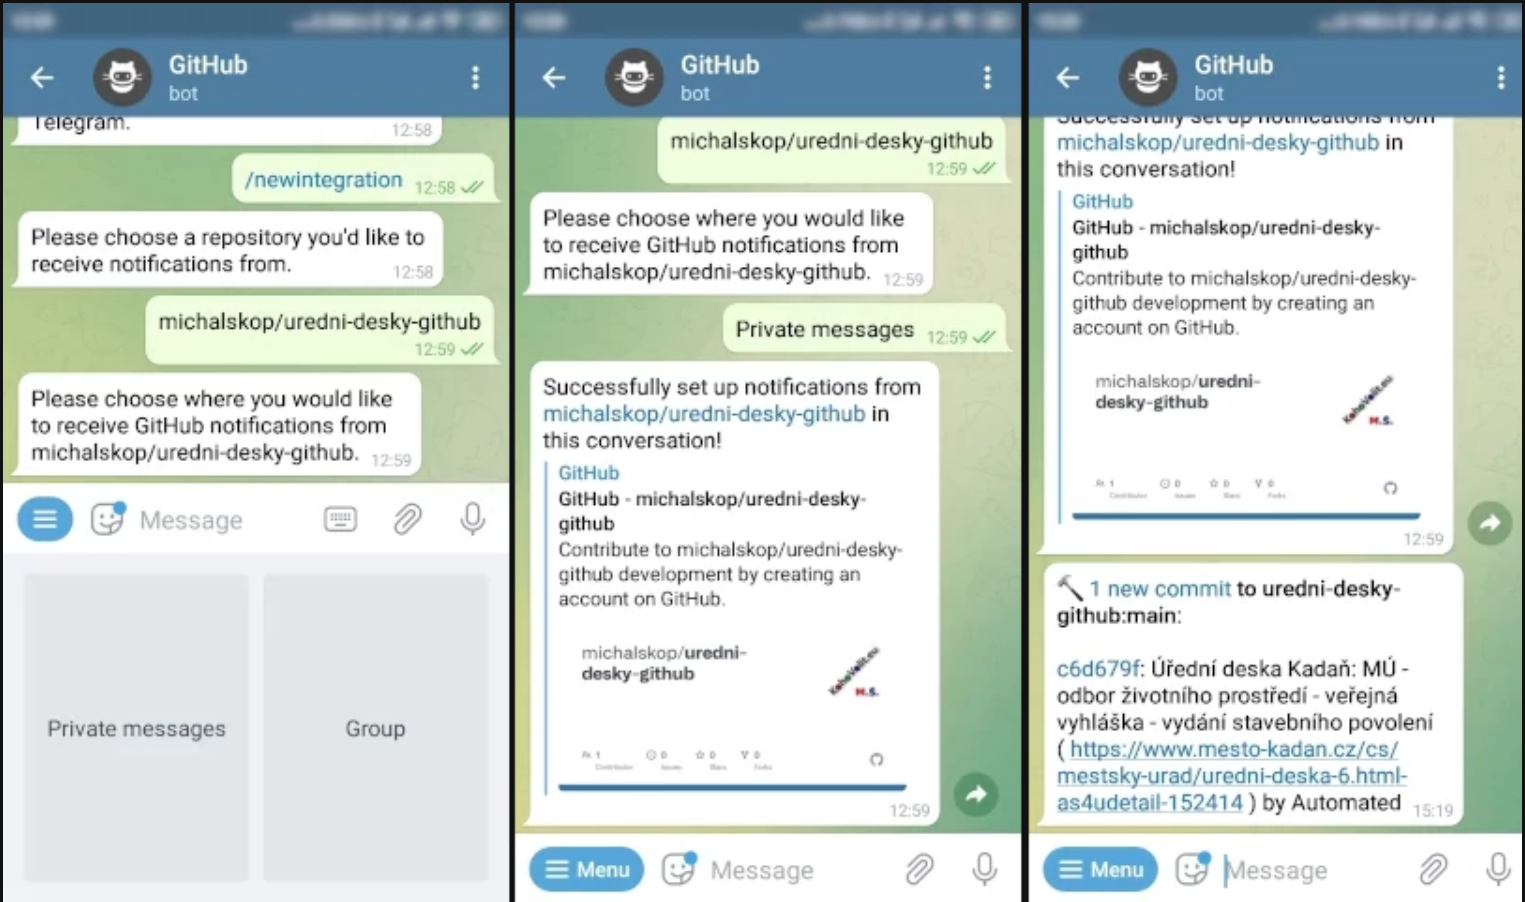
\includegraphics[width=0.85 \linewidth]{img/TelegramNotifikaceUredniDeska.png}
	\caption{Automatické upozornenie, ktoré príde ako textová správa do aplikácie telegram pri pridaní úradnej dosky}
	\label{TelegramNotifikaceUredniDeska}
\end{figure}

\noindent
Tento koncept sa môže použiť práve pri notifikácií obyvateľov, pri zmenách v ich okolí.



\subsection{Projekt edesky.cz}
Projekt edesky zhromažďuje úradné dosky v Českej Republike. Vrámci tohoto zjednotenia poskytuje aj úradne dosky každej mestskej časti Brna\footnote{\url{https://edesky.cz/dokumenty?action=index&controller=documents&hledat_stare=1&zdroj=104}}.


Projekt je tvorený jednotlivcom Marekom Aufartom. Projekt má verejnú dokumentáciu a poskytuje aj API pre vyhľadávanie dokumentov a jednotlivých úradných dosiek.

Aktualita dát má časovú odchýlku pridania na portál rádovo 1-2 hodiny od zverejnenia na oficiálnych stránkach mesta Brna.



%https://edesky.cz/dokumenty?action=index&controller=documents&hledat_stare=1&zdroj=104


\section{Datové sady mesta Brna}
EdeskaBrno - https://edeska.brno.cz/eDeska/



\subsection{Členenie Brna}


Zdroj desek mimo edeska od mesta brna: 

reckovice - \href{http://www.udeska.info/deska.php?login=reckovice}{Reckovice}
oresin - \href{https://www.brno-oresin.cz/uredni-deska.asp}{Oresin}
bystc - \href{https://www.bystrc.cz/uredni-deska.html}{Bystrc}
cervnovice - \href{https://www.cernov.cz/vismo/zobraz_dok.asp?id\_org=2052&id\_ktg=1003}{Cernovice} 

Brno chrlice nemá uredni desky

\href{https://www.mcivanovice.cz/uredni-deska}{Ivanovice}








\section{Otevřená Data}
Open data

\section{Otevřené formální normy}
Od 1.2.2022 je povinnosťou zverejňovať otvorenné dáta podle \cite{ofnUredeniDesky}



\chapter{Analýza}
\label{Analysis}
Táto kapitola sa zamiera na analýzu chybovosti dátových sád, dodržovanie noriem a pod.

\section{system zadavania edesiek}


\section{Analýza edesky.cz}
portál zhromažďuje úspešne 14 z 28 okresov poskytujúcich úradné dosky pre mesto Brno \href{https://edesky.cz/dokumenty?zdroj=104}{tu}. Ostatné dosky majú v svojej kategórii prázdny charakter a okresy Žebetín a Starý Lískovec nemá vo svojej databáze. Časť Brno-Slatina je priradená mimo mesta Brna.

\section{Analýza úradných dosiek podľa metskej časti}

Brno sa skladá z 29 metských častí, z toho dostupné otvorené dáta úradných dosiek sú v nasledujúcej tabuľke \ref{MestskeCastiDostupnost}:

\begin{table}[H]
    \centering
    \begin{tabular}{|l|l|l|l|l|l|}
    \hline
        Mestská časť & číslo & edeska Brno  & Edesky.cz & off. stránka  &  ONF \\ \hline
        Brno-Bohunice & & & \color{green}Áno & \href{https://www.brno-bohunice.cz/cs/urad-mestske-casti/uredni-deska.html}{Bohunice} & ~ \\ \hline
        Brno-Bosonohy & 24 & \color{green}Áno & \color{green}Áno & \href{https://edeska.brno.cz/eDeska24/}{Bosonohy} & ~ \\ \hline
        Brno-Bystrc & & & \color{green}Áno & \href{https://www.bystrc.cz/uredni-deska.html}{Bystrc} & ~\\ \hline
        Brno-Černovice & & & \color{green}Áno& \href{https://www.cernov.cz/vismo/zobraz_dok.asp?id\_org=2052&id\_ktg=1003}{Cernovice}  & ~ \\ \hline
        Brno-Chrlice & & \color{red}Nie& \color{red}Nie & \color{red}Nie & ~ \\ \hline
        Brno-Ivanovice & & & \color{red}Nie& \href{https://www.mcivanovice.cz/uredni-deska}{Ivanovice}& ~ \\ \hline
        Brno-Jehnice & & & \color{green}Áno & \href{http://brno-jehnice.cz/uredni-deska}{Jehnice}& ~ \\ \hline
        Brno-jih & 07 & \color{green}Áno & \color{red}Nie & \href{https://www.brno-jih.cz/uredni-deska/1}{Jih} & ~ \\ \hline
        Brno-Jundrov & & & \color{red}Nie& \href{https://www.jundrov.info/uredni-deska/2}{Jundrov} & ~ \\ \hline
        Brno-Kníničky & 14 & \color{green}Áno & \color{red}Nie & \href{https://edeska.brno.cz/eDeska14/}{Kníničky} &  ~ \\ \hline
        Brno-Kohoutovice & & & \color{red}Nie & \href{https://www.kohoutovice.brno.cz/uredni-deska/2}{Kohoutovice} & ~ \\ \hline
        Brno-Komín & & & \color{green}Áno & \href{https://www.brno-komin.cz/uredni-deska}{Komin}& ~ \\ \hline
        Brno-Královo Pole & 03 & \color{green}Áno & \color{red}Nie & \href{https://kralovopole.brno.cz/uredni-deska/2}{Krpole}& ~ \\ \hline
        Brno-Líšeň & & & \color{red}Nie & \href{https://www.brno-lisen.cz/elektronicka-uredni-deska/s1}{Lisen} & ~ \\ \hline
        Brno-Maloměřice a Obřany & & & \color{red}Nie & \href{https://www.malomerice.cz/uredni-deska/2}{MaO} & ~ \\ \hline
        Brno-Medlánky & 16 & \color{green}Áno & \color{green}Áno & \href{https://edeska.brno.cz//eDeska16/}{Medlanky} & ~ \\ \hline
        Brno-Nový Lískovec & & & \color{red}Nie & \href{https://www.novy-liskovec.cz/uredni-deska/2}{NLiskovec}  & ~ \\ \hline
        Brno-Ořešín & &  & \color{green}Áno & \href{https://www.brno-oresin.cz/uredni-deska.asp}{Oresin}& ~ \\ \hline
        Brno-Řečkovice a Mokrá Hora & & & \color{green}Áno & \href{http://www.udeska.info/deska.php?login=reckovice}{Reckovice}& ~ \\ \hline
        Brno-sever & 04 & \color{green}Áno & \color{red}Nie & \href{https://www.sever.brno.cz/uredni-deska.html}{Sever}& ~ \\ \hline
        Brno-Slatina & & & \color{green}Áno& \href{https://www.mcslatina.cz/uredni-deska}{Slatina} & ~ \\ \hline
        Brno-Starý Lískovec & & & \color{red}Nie & \href{https://www.staryliskovec.cz/cs/urad/uredni-deska-1.html}{SLiskovec} & ~ \\ \hline
        Brno-střed & 01 & \color{green}Áno & \color{red}Nie & \href{https://edeska.brno.cz/eDeska01/}{Stred} & ~ \\ \hline
        Brno-Tuřany & & & \color{green}Áno & \href{https://www.turany.cz/uredni-deska/}{Turany}& ~ \\ \hline
        Brno-Útěchov & & & \color{green}Áno & \href{https://brno-utechov.cz/category/uredni-deska/}{Utechov}& ~ \\ \hline
        Brno-Vinohrady & & & \color{green}Áno & \href{https://www.vinohrady.brno.cz/urad/uredni-deska}{Utechov} & ~ \\ \hline
        Brno-Žabovřesky & & & \color{red}Nie & \href{https://www.zabovresky.cz/uredni-deska/1}{Zabovresky} & ~ \\ \hline
        Brno-Žebětín & & & \color{green}Áno & \href{https://www.zebetin.cz/uredni-deska/2}{Zebetin} & ~ \\ \hline
        Brno-Židenice & 05 & \color{green}Áno & \color{red}Nie & \href{https://edeska.brno.cz/eDeska05/}{Zidenice}& ~ \\ \hline
    \end{tabular}
    \label{MestskeCastiDostupnost}
    \caption{Tabuľka zobrazuje dostupnosť jednotlivých zdrojov na podporovaných portáloch a ich zastúpnie v Otvorenej Normálnej Forme.}
\end{table}

\chapter{Návrh}
\label{Concept}

\chapter{Implementácia}
